%%%%%%%%%%%%%%%%%%%%%%%%%%%%%%%%%%%%%%%%%
% Classicthesis Typographic Thesis
% LaTeX Template
% Version 1.3 (15/2/14)
%
% This template has been downloaded from:
% http://www.LaTeXTemplates.com
%
% Original author:
% André Miede (http://www.miede.de)
%
% License:
% CC BY-NC-SA 3.0 (http://creativecommons.org/licenses/by-nc-sa/3.0/)
%
% General Tips:
% 1) Make sure to edit the classicthesis-config.file
% 2) New enumeration (A., B., C., etc in small caps): \begin{aenumerate} \end{aenumerate}
% 3) For margin notes: \marginpar or \graffito{}
% 4) Do not use bold fonts in this style, it is designed around them
% 5) Use tables as in the examples
% 6) See classicthesis-preamble.sty for useful commands
%
%%%%%%%%%%%%%%%%%%%%%%%%%%%%%%%%%%%%%%%%%

%----------------------------------------------------------------------------------------
%	PACKAGES AND OTHER DOCUMENT CONFIGURATIONS
%----------------------------------------------------------------------------------------

\documentclass[
		oneside,openright,titlepage,numbers=noenddot,headinclude,%1headlines,
                footinclude=true,cleardoublepage=empty,
                BCOR=5mm,paper=a4,fontsize=11pt, % Binding correction, paper type and font size
                norsk, % Languages
                ]{scrreprt} 
                
% Includes the file which contains all the document configurations and packages - make sure to edit this file
%%%%%%%%%%%%%%%%%%%%%%%%%%%%%%%%%%%%%%%%%
% Thesis Configuration File
%
% The main lines to change in this file are in the DOCUMENT VARIABLES
% section, the rest of the file is for advanced configuration.
%
%%%%%%%%%%%%%%%%%%%%%%%%%%%%%%%%%%%%%%%%%

%----------------------------------------------------------------------------------------
%	DOCUMENT VARIABLES
%	Fill in the lines below to enter your information into the thesis template
%	Each of the commands can be cited anywhere in the thesis
%----------------------------------------------------------------------------------------

% Remove drafting to get rid of the '[ Date - classicthesis version 4.0 ]' text at the bottom of every page
\PassOptionsToPackage{eulerchapternumbers,listings, pdfspacing, subfig,beramono,eulermath,parts,dottedtoc}{classicthesis}
% Available options: drafting parts nochapters linedheaders eulerchapternumbers beramono eulermath pdfspacing minionprospacing tocaligned dottedtoc manychapters listings floatperchapter subfig
% Adding 'dottedtoc' will make page numbers in the table of contents flushed right with dots leading to them

\newcommand{\myTitle}{Prosjektrapport\xspace}
\newcommand{\mySubtitle}{Robot og Menneske\xspace}
\newcommand{\myDegree}{Engineering student\xspace}
\newcommand{\myGroup}{4\xspace}
\newcommand{\myName}{Helene Myre\\Erlend Hestnes\\Jon Zwaig Kolstad\\Morten Mjelva\\Harald Moholt\\H\r{a}vard Mo\r{a}s\xspace}
\newcommand{\myProf}{\xspace}
\newcommand{\myOtherProf}{\xspace}
\newcommand{\mySupervisor}{\xspace}
\newcommand{\myFaculty}{Faculty of Information Technology, Mathematics and Electrical Engineering\xspace}
\newcommand{\myDepartment}{Department of Engineering Cybernetics\xspace}
\newcommand{\myUni}{Norwegian University of Science and Technology\xspace}
\newcommand{\myLocation}{Trondheim\xspace}
\newcommand{\myTime}{April 2015\xspace}
\newcommand{\myVersion}{version 4.0\xspace}

%----------------------------------------------------------------------------------------
%	USEFUL COMMANDS
%----------------------------------------------------------------------------------------

\newcommand{\ie}{i.\,e.}
\newcommand{\Ie}{I.\,e.}
\newcommand{\eg}{e.\,g.}
\newcommand{\Eg}{E.\,g.} 

\newcounter{dummy} % Necessary for correct hyperlinks (to index, bib, etc.)
\providecommand{\mLyX}{L\kern-.1667em\lower.25em\hbox{Y}\kern-.125emX\@}

%----------------------------------------------------------------------------------------
%	PACKAGES
%----------------------------------------------------------------------------------------

\usepackage{lipsum} % Used for inserting dummy 'Lorem ipsum' text into the template

%------------------------------------------------
 
\PassOptionsToPackage{utf8}{inputenc}
\usepackage{inputenc}
 
 %------------------------------------------------

\PassOptionsToPackage{norsk}{babel}  % Change this to your language(s)
% Spanish languages need extra options in order to work with this template
%\PassOptionsToPackage{spanish,es-lcroman}{babel}
\usepackage{babel}

%------------------------------------------------			

\PassOptionsToPackage{square,numbers}{natbib}
 \usepackage{natbib}
 
 %------------------------------------------------

\PassOptionsToPackage{fleqn}{amsmath} % Math environments and more by the AMS 
 \usepackage{amsmath}
 
 %------------------------------------------------

\PassOptionsToPackage{T1}{fontenc} % T2A for cyrillics
\usepackage{fontenc}

%------------------------------------------------

\usepackage{xspace} % To get the spacing after macros right

%------------------------------------------------

\usepackage{mparhack} % To get marginpar right

%------------------------------------------------

\usepackage{fixltx2e} % Fixes some LaTeX stuff 

%------------------------------------------------

\usepackage{parskip}

%------------------------------------------------

\usepackage{babel}

%------------------------------------------------

\PassOptionsToPackage{smaller}{acronym} % Include printonlyused in the first bracket to only show acronyms used in the text
\usepackage{acronym} % nice macros for handling all acronyms in the thesis

%------------------------------------------------

%\renewcommand*{\acsfont}[1]{\textssc{#1}} % For MinionPro
%\renewcommand{\bflabel}[1]{{#1}\hfill} % Fix the list of acronyms

%------------------------------------------------

\PassOptionsToPackage{pdftex}{graphicx}
\usepackage{graphicx} 

%---------------------------------------------------------------------------------------- 
%	FLOATS: TABLES, FIGURES AND CAPTIONS SETUP
%----------------------------------------------------------------------------------------

\usepackage{tabularx} % Better tables
\setlength{\extrarowheight}{3pt} % Increase table row height
\newcommand{\tableheadline}[1]{\multicolumn{1}{c}{\spacedlowsmallcaps{#1}}}
\newcommand{\myfloatalign}{\centering} % To be used with each float for alignment
\usepackage{caption}
\captionsetup{format=hang,font=small}
\usepackage{subfig}  

%----------------------------------------------------------------------------------------
%	CODE LISTINGS SETUP
%----------------------------------------------------------------------------------------

\usepackage{listings} 
%\lstset{emph={trueIndex,root},emphstyle=\color{BlueViolet}}%\underbar} % for special keywords
\lstset{language=[LaTeX]Tex, % Specify the language for listings here
keywordstyle=\color{RoyalBlue}, % Add \bfseries for bold
basicstyle=\small\ttfamily, % Makes listings a smaller font size and a different font
%identifierstyle=\color{NavyBlue}, % Color of text inside brackets
commentstyle=\color{Green}\ttfamily, % Color of comments
stringstyle=\rmfamily, % Font type to use for strings
numbers=left, % Change left to none to remove line numbers
numberstyle=\scriptsize, % Font size of the line numbers
stepnumber=5, % Increment of line numbers
numbersep=8pt, % Distance of line numbers from code listing
showstringspaces=false, % Sets whether spaces in strings should appear underlined
breaklines=true, % Force the code to stay in the confines of the listing box
%frameround=ftff, % Uncomment for rounded frame
frame=single, % Frame border - none/leftline/topline/bottomline/lines/single/shadowbox/L
belowcaptionskip=.75\baselineskip % Space after the "Listing #: Desciption" text and the listing box
}

%----------------------------------------------------------------------------------------
%	HYPERREFERENCES
%----------------------------------------------------------------------------------------

\PassOptionsToPackage{pdftex,hyperfootnotes=false,pdfpagelabels,backref}{hyperref}
\usepackage{hyperref}  % backref linktocpage pagebackref
\pdfcompresslevel=9
\pdfadjustspacing=1

\hypersetup{
% Uncomment the line below to remove all links (to references, figures, tables, etc)
%draft, 
%colorlinks=true, linktocpage=true, linktoc=all, pdfstartpage=1, pdfstartview=FitV,
% Uncomment the line below if you want to have black links (e.g. for printing black and white)
colorlinks=false, linktocpage=false, pdfborder={0 0 0}, pdfstartpage=1, pdfstartview=FitV, 
breaklinks=true, pdfpagemode=UseNone, pageanchor=true, pdfpagemode=UseOutlines,
plainpages=false, bookmarksnumbered, bookmarksopen=true, bookmarksopenlevel=1,
hypertexnames=true, pdfhighlight=/O, urlcolor=webbrown, linkcolor=RoyalBlue, citecolor=webgreen,
%------------------------------------------------
% PDF file meta-information
pdftitle={\myTitle},
pdfauthor={\textcopyright\ \myName, \myUni, \myFaculty},
pdfsubject={},
pdfkeywords={},
pdfcreator={pdfLaTeX},
pdfproducer={LaTeX with hyperref and classicthesis}
%------------------------------------------------
}   

%----------------------------------------------------------------------------------------
%	BACKREFERENCES
%----------------------------------------------------------------------------------------

\usepackage{ifthen} % Allows the user of the \ifthenelse command
\newboolean{enable-backrefs} % Variable to enable backrefs in the bibliography
\setboolean{enable-backrefs}{false} % Variable value: true or false

\newcommand{\backrefnotcitedstring}{\relax} % (Not cited.)
\newcommand{\backrefcitedsinglestring}[1]{(Cited on page~#1.)}
\newcommand{\backrefcitedmultistring}[1]{(Cited on pages~#1.)}
\ifthenelse{\boolean{enable-backrefs}} % If backrefs were enabled
{
\PassOptionsToPackage{hyperpageref}{backref}
\usepackage{backref} % to be loaded after hyperref package 
\renewcommand{\backreftwosep}{ and~} % separate 2 pages
\renewcommand{\backreflastsep}{, and~} % separate last of longer list
\renewcommand*{\backref}[1]{}  % disable standard
\renewcommand*{\backrefalt}[4]{% detailed backref
\ifcase #1 
\backrefnotcitedstring
\or
\backrefcitedsinglestring{#2}
\else
\backrefcitedmultistring{#2}
\fi}
}{\relax} 

%----------------------------------------------------------------------------------------
%	AUTOREFERENCES SETUP
%	Redefines how references in text are prefaced for different 
%	languages (e.g. "Section 1.2" or "section 1.2")
%----------------------------------------------------------------------------------------

\makeatletter
\@ifpackageloaded{babel}
{
\addto\extrasnorsk{
\renewcommand*{\figureautorefname}{Figur}
\renewcommand*{\tableautorefname}{Tabell}
\renewcommand*{\partautorefname}{Del}
\renewcommand*{\chapterautorefname}{Kapittel}
\renewcommand*{\sectionautorefname}{Delkapittel}
\renewcommand*{\subsectionautorefname}{Delkapittel}
\renewcommand*{\subsubsectionautorefname}{Delkapittel}
\renewcommand*{\appendixautorefname}{Vedlegg}
}
\addto\extrasngerman{
\renewcommand*{\paragraphautorefname}{Absatz}
\renewcommand*{\subparagraphautorefname}{Unterabsatz}
\renewcommand*{\footnoteautorefname}{Fu\"snote}
\renewcommand*{\FancyVerbLineautorefname}{Zeile}
\renewcommand*{\theoremautorefname}{Theorem}
\renewcommand*{\appendixautorefname}{Anhang}
\renewcommand*{\equationautorefname}{Gleichung}
\renewcommand*{\itemautorefname}{Punkt}
}
\providecommand{\subfigureautorefname}{\figureautorefname} % Fix to getting autorefs for subfigures right
}{\relax}
\makeatother

%----------------------------------------------------------------------------------------

\usepackage{classicthesis}

%------------------------------------------------

\usepackage{todonotes}

%----------------------------------------------------------------------------------------
%	CHANGING TEXT AREA 
%----------------------------------------------------------------------------------------

%\linespread{1.05} % a bit more for Palatino
%\areaset[current]{312pt}{761pt} % 686 (factor 2.2) + 33 head + 42 head \the\footskip
%\setlength{\marginparwidth}{7em}%
%\setlength{\marginparsep}{2em}%

%----------------------------------------------------------------------------------------
%	USING DIFFERENT FONTS
%----------------------------------------------------------------------------------------

%\usepackage[oldstylenums]{kpfonts} % oldstyle notextcomp
%\usepackage[osf]{libertine}
%\usepackage{hfoldsty} % Computer Modern with osf
%\usepackage[light,condensed,math]{iwona}
%\renewcommand{\sfdefault}{iwona}
%\usepackage{lmodern} % <-- no osf support :-(
%\usepackage[urw-garamond]{mathdesign} <-- no osf support :-(

\let\marginpar\oldmarginpar

\begin{document}

\frenchspacing % Reduces space after periods to make text more compact

\raggedbottom % Makes all pages the height of the text on that page

\selectlanguage{norsk} % Select your default language - e.g. american or ngerman

%\renewcommand*{\bibname}{new name} % Uncomment to change the name of the bibliography
%\setbibpreamble{} % Uncomment to include a preamble to the bibliography - some text before the reference list starts

\pagenumbering{roman} % Roman page numbering prior to the start of the thesis content (i, ii, iii, etc)

\pagestyle{plain} % Suppress headers for the pre-content pages

%----------------------------------------------------------------------------------------
%	PRE-CONTENT THESIS PAGES
%----------------------------------------------------------------------------------------

% Title Page

\begin{titlepage}

%\begin{addmargin}[-1cm]{-3cm}
\begin{center}
\large

\hfill
\vfill

\begingroup
\color{Maroon}\spacedallcaps{\myTitle} \\ \bigskip % Thesis title
\endgroup

% Additional Information about the document
\begin{minipage}{0.4\textwidth}
    \centering
	\large
		\emph{Gruppe \myGroup:}\\~\\
		\myName
\end{minipage}
\vfill

%\includegraphics[width=6cm]{gfx/logo} \\ \medskip % Picture

\mySubtitle \\ \medskip % Thesis subtitle
%\myDegree \\
%\myDepartment \\
%\myFaculty \\
%\myUni \\ \bigskip

\myTime

\vfill

\end{center}
%\end{addmargin}

\end{titlepage} % Main title page

\cleardoublepage% Abstract

\pdfbookmark[1]{Sammendrag}{Sammendrag} % Bookmark name visible in a PDF viewer

\begingroup
\let\clearpage\relax
\let\cleardoublepage\relax
\let\cleardoublepage\relax

\chapter*{Sammendrag} % Abstract name
 Robotikk er i stadig større grad brukt i industri, men er fremdeles i liten
grad benyttet for å lette menneskers daglige liv. Autonome handlevogner vil
kunne være til stor hjelp blant annet for eldre eller handicappede brukere,
eller i situasjoner der kunder må transportere tunge varer.
Vi foreslår en automatisert handlevogn som følger en kunde rundt i butikken,
og transporterer varer for kunden mens han eller hun handler.
Den følgende artikkelen beskriver en implementasjon av en automatisert
handlevogn. Vi foreslår en løsning bestående av et eksternt
posisjoneringssystem som sammen med lokale sensorer muliggjør navigasjon. Løsningen er realisert ved et OptiTrack motion capture
kamerasystem og en MobileRobots Pioneer P3-DX, med et sonararray og en
laseravstandsmåler, styrt av Robot Operating System.
Resultater av testing på en prototype viser at en slik løsning muliggjør
navigasjon i den type uoversiktlige omgivelser man vil finne i et realistisk
scenario med høy grad av sikkerhet og presisjon.
\endgroup			

\vfill % Abstract page

\pagestyle{scrheadings} % Show chapter titles as headings

\cleardoublepage% Table of Contents - List of Tables/Figures/Listings and Acronyms

\refstepcounter{dummy}

\pdfbookmark[1]{\contentsname}{tableofcontents} % Bookmark name visible in a PDF viewer

\setcounter{tocdepth}{2} % Depth of sections to include in the table of contents - currently up to subsections

\setcounter{secnumdepth}{3} % Depth of sections to number in the text itself - currently up to subsubsections

\manualmark
\markboth{\spacedlowsmallcaps{\contentsname}}{\spacedlowsmallcaps{\contentsname}}
\tableofcontents 
\automark[section]{chapter}
\renewcommand{\chaptermark}[1]{\markboth{\spacedlowsmallcaps{#1}}{\spacedlowsmallcaps{#1}}}
\renewcommand{\sectionmark}[1]{\markright{\thesection\enspace\spacedlowsmallcaps{#1}}}

\clearpage

\begingroup 
\let\clearpage\relax
\let\cleardoublepage\relax
\let\cleardoublepage\relax

%----------------------------------------------------------------------------------------
%	List of Figures
%----------------------------------------------------------------------------------------

\refstepcounter{dummy}
%\addcontentsline{toc}{chapter}{\listfigurename} % Uncomment if you would like the list of figures to appear in the table of contents
\pdfbookmark[1]{\listfigurename}{lof} % Bookmark name visible in a PDF viewer

\listoffigures

\vspace*{8ex}
\newpage

%----------------------------------------------------------------------------------------
%	List of Tables
%----------------------------------------------------------------------------------------

%\refstepcounter{dummy}
%\addcontentsline{toc}{chapter}{\listtablename} % Uncomment if you would like the list of tables to appear in the table of contents
%\pdfbookmark[1]{\listtablename}{lot} % Bookmark name visible in a PDF viewer

%\listoftables
        
%\vspace*{8ex}
%\newpage
    
%----------------------------------------------------------------------------------------
%	List of Listings
%---------------------------------------------------------------------------------------- 

%\refstepcounter{dummy}
%\addcontentsline{toc}{chapter}{\lstlistlistingname} % Uncomment if you would like the list of listings to appear in the table of contents
%\pdfbookmark[1]{\lstlistlistingname}{lol} % Bookmark name visible in a PDF viewer

%\lstlistoflistings 

%\vspace*{8ex}
%\newpage
       
%----------------------------------------------------------------------------------------
%	Acronyms
%----------------------------------------------------------------------------------------

\refstepcounter{dummy}
%\addcontentsline{toc}{chapter}{Acronyms} % Uncomment if you would like the acronyms to appear in the table of contents
\pdfbookmark[1]{Forkortelser}{forkortelser} % Bookmark name visible in a PDF viewer

\markboth{\spacedlowsmallcaps{Acronyms}}{\spacedlowsmallcaps{Acronyms}}

\chapter*{Forkortelser}

\begin{acronym}[SLAM]
\acro{API}{Application Programmers Interface}
\acro{ARIA}{Advanced Robot Interface for Applications}
\acro{ROS}{Robot Operating System}
\acro{SLAM}{Simultaneous Localization And Mapping}
\end{acronym}  
                   
\endgroup % Contents, list of figures/tables/listings and acronyms

\cleardoublepage

\pagenumbering{arabic} % Arabic page numbering for thesis content (1, 2, 3, etc)
%\setcounter{page}{90} % Uncomment to manually start the page counter at an arbitrary value (for example if you wish to count the pre-content pages in the page count)

\cleardoublepage % Avoids problems with pdfbookmark

%----------------------------------------------------------------------------------------
%	THESIS CONTENT - CHAPTERS
%----------------------------------------------------------------------------------------

\listoftodos

\part{Rapport} % First part of the thesis

% Innledning

\chapter{Innledning} % Chapter title

\label{ch:innledning} % For referencing the chapter elsewhere, use \autoref{ch:introduction} 
%----------------------------------------------------------------------------------------

Denne prosjektrapporten er skrevet i forbindelse med gruppe 4 sitt arbeid i emnet TTK4851 Eksperter i Team, landsby for Robotikk og Menneske. Arbeidet foregikk våren 2015, fra oppstart 7. januar, til levering 29. april. I dette kapittelet fokuseres det på bakgrunn, motivasjon, begrensninger, bidrag og videre disposisjon av oppgaven. 

\section{Bakgrunn for oppgaven}

%\begin{itemize}
%\item Hva er behovet?
%\item Hvordan har oppgaven vært løst tidligere?
%\item Hvordan går vårt prosjekt inn i "den store sammenhengen"?
%\item Hva bygger dette prosjektet på (for eksempel en masteroppgave, et konkret annet arbeid)
%\end{itemize}

\subsection{Behov}

En autonom robot er en plattform med mange bruksområder. Denne rapporten ser på mulighetene med å erstatte den tradisjonelle handlevognen med en robot. På denne måten slipper kunden å dytte rundt på vognen sin selv. Til korte handleturer med lette eller små varer vil det ikke være noe særlig behov for en slik robot, da en kurv eller vogn kan gjøre jobben billigere og bedre. Hvis man derimot skal handle større eller tyngre varer, f.eks. på IKEA eller store varehus, kan en robot gjøre handleprosessen mye enklere. Det er også særlig i tilfeller hvor personen som handler er handikappet, gammel eller på annen måte er i dårlig stand til å trille eller bære varer selv, en butikkrobot vil være til mye hjelp. 

\subsection{Tidligere arbeid}
Innenfor verden av roboter og droner har det i de siste årene blitt en økende trend i roboter som beveger seg rundt av seg selv. I artikkelen til ukebladet Wired \citep{next_big_trend} kan en lese om roboter som følger mennesker ved hjelp av ultralydsensorer eller lys-sensorer. For å unngå hindringer er det både eksperimentert med lasersensorer og ultrasoniske løsninger, samt tredimensjonal kartlegging ved bruk av laser. Robotene, som artikkelen omtaler, er planlagt å kunne brukes kommersielt. Eksempel på oppgaver er lagerarbeid ved varehus og fabrikker, caddy på en golfbane og ved jordbruks- og industrimiljøer.

\subsection{Den store sammenhengen}
En rekke aktører har allerede utviklet roboter som følger etter deg og bærer ting for deg. Disse robotene er vanligvis dyre, og som regel forbeholdt sektorer som industri og helse. Vi ønsker derimot å presentere et forslag til forbrukerne, nemlig en robot som skal kunne brukes av kunden i en butikk eller et varehus. Det er derfor viktig at løsningen passer i slike lokaler, og at den heller ikke har for store kostnader. Prisen på produktet er svært viktig, ettersom butikker i dag ikke bruker mange kroner på en vanlig handlevogn. %Det er også viktig å presisere at den løsningen som blir presentert i denne rapporten kun er en prototype, og ikke et ferdig produkt.

\section{Motivasjon}
Det har alltid vært et mål for gruppen å kunne bruke de respektive fagfeltene til hvert enkelt gruppemedlem, for deretter å bruke denne kompetansen til å få et best mulig produkt. Halvparten av gruppemedlemmene var personer med utdanning innen teknisk kybernetikk, mens resten av medlemmene satt med teknisk kunnskap fra andre retninger. Dette gjorde at vi hadde gode forutsetninger til å kunne gjøre noe praktisk i løpet av arbeidsperioden. Gruppesammensetningen er derfor en viktig årsak til at vi som gruppe havnet på ideen om å lage en menneskefølgende butikk-robot. I tillegg til kompetansen som lå til grunn i gruppa, var det også en stor enighet om at det var en oppgave som kunne være morsom å gjennomføre.

\section{Begrensninger}
%\begin{itemize}
%\item Har vi fokusert på biter av oppgaven?
%\item Har det vært ressursbegrensninger som gjør at vi ikke har gjort ideelle valg?
%\end{itemize}

\subsection{Oppdeling av oppgave}
Vi har fra dag én hatt et stort fokus på å gjøre oppgaven så modulær som mulig. Stifinning, sensorer, kollisjon-deteksjon og robot-kontroll ble naturlige biter i et større puslespill. Fokuset på gjøre prosjektet modulært kom først og fremst fra ønsket om å kunne jobbe parallelt med ulike deler. Det var fra starten av veldig høyt fokus på at disse skulle kunne jobbes med selvstendig og uavhengig, men på grunn av begrensninger på utstyr ble gruppen tvunget til å smelte bitene sammen.

\subsection{Robot}
Til dette prosjektet, fikk gruppen tilgang på én utviklingsrobot av typen Pioneer 3-DX. Dette har vært problematisk for gruppen, da en hele tiden har hatt et ønske om å kunne jobbe parallelt med både stifinning, sensorer, kollisjon-deteksjon og robot-kontroll. Roboten og sensorene lar bare én datamaskin være tilkoblet om gangen, så hvis noen ønsket å jobbe med forskjellige oppgaver, ble gruppen nødt til å vente på tur for å kunne teste løsningene. Gruppen har jobbet rundt begrensningene ved å lese og lære om teknologiene og metodene som kan brukes på forhånd av faktisk utvikling, men det hadde definitivt vært enklere om det hadde vært tilgang på mer utstyr.

\subsection{Kompetanse}
Til tross for at var flere på gruppen som hadde relevant kompetanse innenfor både robotikk og programvare, så var hadde det ingen som hadde erfaring med Pioneer 3-DX eller robot operativsystemet (ROS). Vi fikk også inntrykk av at det ikke var så mange på universitetet som hadde god erfaring med roboten. Alt dette medførte at gruppen brukte mye tid på å bli kjent med utstyret og gjennomføre opplæring av hverandre. 

\subsection{Tid}
Eksperter i team er et prosjekt med begrenset tid, og det er derfor vanskelig å kunne ferdigstille et avansert teknisk produkt på den tiden som er avsatt. I tillegg til dårlig tid, er det også kun avsatt onsdager for å jobbe med emnet. Mye blir glemt på en uke, noe som gjør at en må bruke en del tid hver landsbydag på å komme inn i det man gjorde forrige gang. Denne oppgaven hadde uten tvil vært enklere hvis landsbydagene hadde vært sammenhengene. 

% Litt usikker på hvor dette kommer fra ---> %Før den endelige planen for gjennomføringen av prosjektet ble bestemt, var det flere mulige andre metoder som ble diskutert for å hente posisjonsdata. I utgangspunktet hadde gruppen valgt å finne posisjon ved hjelp av Bluetooth beacons ved å triangulere signalet. Bruk av signalstyrke for å finne avstand var en mulighet, men for unøyaktig for denne typen bruk. En annen metode er å bruke fasen til signalet for å avgjøre avstanden og dermed posisjon. Denne metoden var utilgjengelig for gruppen og kunne ikke anvendes. 

\section{Bidrag}
%Kort oppsummering av det nye / smarte som er gjort.
Vårt bidrag er en prototype og ikke et ferdigstilt produkt. Prototypen er en autonom robot som bruker et avansert infrarødt kamerasystem for å kunne plassere et menneske og en robot i rommet. Koordinater til person og robot blir behandlet slik at roboten kan følge etter mennesket. Roboten har også en laser-scanner som kan kartlegge omgivelsene og detektere objekter rundt seg. Hvis objekter er et hinder for roboten vil den finne veien til målet uten å skade seg selv eller objektet. 

\section{Disposisjon av oppgaven}
\todo[caption=Disposisjon]{Disposisjon av oppgaven: Se over at dette stemmer overens før levering}
% Kort (1 – 3 setninger) om hva som er i hvert kapittel.

% \paragraph{Litteraturstudie} Formålet med dette kapittelet av rapporten er å kunne vise til kunnskap og informasjonskilder gruppen har brukt igjennom prosjektiden. Dette vil være en oppsummering av alle litteraturkilder og forklare hva vi tok med oss videre.

\paragraph{Teori} Formålet med dette kapittelet er å gjøre rede for tidligere arbeid innenfor fagfeltet og samle bakgrunnsinformasjon som er nødvendig for å forstå det arbeidet som utføres i oppgaven. Kapittelet inneholder fagrelatert informasjon og tekniske begreper som brukes i løsning og implementasjon.

\paragraph{Løsning} Hensikten med dette kapittelet er å presentere ideen, krav\-ene og målene gruppen satte seg. 

\paragraph{Implementasjon} Formålet med dette kapittelet er å presentere vår implementasjon av løsningene av kravene vi skulle oppnå. Dette kapittelet vil også inneholde begrunnelser for valg.

\paragraph{Resultater} Formålet med dette kapittelet er å ta for oss målene og resultater som viser til at vi har oppnådd kravene til oppgaven.

\paragraph{Diskusjon} Formålet med dette kapittelet er å diskutere resultat\-ene, først og fremst mot teori og implementasjon.

\paragraph{Konklusjon} I dette kapittelet ønsker vi å uttrykke konklusjonene for vårt system.

\paragraph{Videre arbeid} I dette kapittelet vil vi legge frem mulig videre arbeid og hva som eventuelt må gjøres før dette kan iverksettes. % Innledning
%% Litteratur

\chapter{Litteratur} % Chapter title

\label{ch:litteratur} % For referencing the chapter elsewhere, use \autoref{ch:background}
%----------------------------------------------------------------------------------------

\todo{Fjerne hele litteraturstudie og sammenfatt med teori-delen?}

Den essensielle teknologiske leveransen fra prosjektet er ikke radikalt ny. Det vil si at noen har fått denne ideen og uvtiklet den tidligere. Prosjektet har både konkurrenter som løser  , men også komponentene som systemet skal bestå av. 
\\
Hva har andre gjort for å løse "vårt" eller tilsvarende / lignende problem? Kort innledning.
\section{Funn 1}
Funn, funn, gull bar-dunn.
\section{Funn 2}
Funn, svunn, barkinn og starmunn. 
\section{Oppsummering av litteraturstudiet}
Oppsummering.

SLAM - Sim. Localis. and Modeling % Litteraturstudie
% Teori

\chapter{Teori} % Chapter title

\label{ch:teori} % For referencing the chapter elsewhere, use \autoref{ch:mathtest}

% Formålet med dette kapittelet er å gjøre rede for tidligere arbeid innenfor fagfeltet og samle bakgrunnsinformasjon som er nødvendig for å forstå det arbeidet som utføres i oppgaven. Kapittelet inneholder
% fagrelatert informasjon og tekniske begreper som brukes i løsning og implementasjon.
%----------------------------------------------------------------------------------------

\section{Pioneer P3-DX}

Pioneer P3-DX er en robot levert av Adept MobileRobots. Den er sett på som pålitelig, og derfor ofte brukt i forbindelse med forskning og eksperimenter. Roboten kommer som standard med to styrbare 19 cm hjul, et lite, passivt støttehjul, og 8 sonarsensorer montert foran, og tilsvarende bak. I tillegg er det på utgaven som ITK besitter montert et forriglingssystem i form av kontaktsensorer, også kalt <<bumper>>-sensorer, langs hele kanten foran og bak. På toppen av roboten er det en flat plattform, perfekt for montasje av annet utstyr. 

Roboten har en egen innebygget kontroller for styring, tilgjengelig via seriellport. For å kontrollere roboten via ROS benyttes det en driver som sender kommanodoer til robotens grensesnitt, ARIA\footnote{\url{http://robots.mobilerobots.com/wiki/ARIA}}. ARIA, eller Advanced Robot Interface for Applications, lar brukeren kontrollere robotens fart og retning, lese av sensorverdier og så videre.

\begin{figure}[h!]
  \centering
    \reflectbox{%
      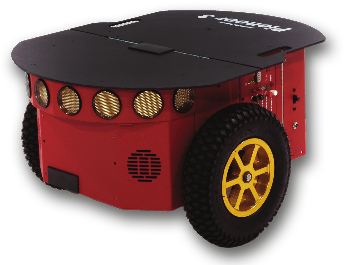
\includegraphics[width=0.5\textwidth]{gfx/pioneer3dx_real.png}}
  \caption{Pioneer P3-DX}
  \label{fig:pioneer}
\end{figure}

\section{ROS}

ROS (Robot Operating System) er et fleksibelt rammeverk for styring av roboter. Rammeverket har fokus på brukervennlighet og robusthet, og er ikke spesifikt for én type robot. ROS har derfor gjort seg svært egnet for dette prosjektet. Operativsystemet er bygget opp av moduler som sender og mottar informasjon via meldingskanaler. Dette letter implementasjon av de enkelte modulene, da de får tydelige grensesnitt som gjør at de kan testes uavhengig av andre moduler.

\section{Flex 13 og Motion Capture Systems}

Flex 13 er et infrarødt kamera, levert av OptiTrack\footnote{\url{https://www.optitrack.com/}}. Markører, i form av kuler med en spesiell overflate, reflekterer de infrarøde strålene tilbake slik at de oppdages av kameraet. Ved å lage bestemte mønstre med slike kuler, og bruke samme type kamera i forskjellige vinkler er det mulig å danne svært nøyaktige tredimensjonale inntrykk av fysiske objekter. Et slikt system er et eksempel på et <<Motion Capture System>>, og da brukes det til å spore bevegelsene til objekter. Data fra et slik system kan brukes til mange forskjellige formål, og avhenger helt av kompleksiteten til objektet som spores. 


% Et  «Motion  Capture»  system  har  blitt  brukt  som  posisjoneringssys-tem for dette prosjektet. Kamerasystemet består av rekke takmontereinfrarøde kamera som er i stand å fange opp refleksjoner fra spesiellemarkører nede på bakken. Ved bruk av skreddersydd programvare erdette systemet i stand til å kalkulere kartesiske koordinater med millimeterpresisjon for de gitte markørene og sende disse koordinatene utpå en strøm. 


\section{Motive}

Motive er en programvare pakke fra OptiTrack. Programmet henter data fra de infrarøde kameraene, og presenterer et tredimensjonalt bilde over markørene som befinner seg innenfor kameraenes synsområde.
Disse kan grupperes og defineres som legemer, og programmet kan deretter spore både posisjon og orientasjon for hvert legeme. Bevegelsene til legemene kan lagres for senere analyse, eller de kan overføres 
til andre datamaskiner på nettverket.

\section{Stifinning}

Stifinning er tilnærmingen på å finne korteste vei fra ett punkt til et annet. Det er mange måter å gjennomføre dette på, og avhenger helt av miljøet hvor det skjer og hvilke data som er og blir tilgjengelig. Et praktisk problem kan f.eks. være å sammenlikne forskjellige ruter for en bil som skal frakte varer fra by A til by B. Basert på kunnskap om fartsgrenser og avstander vil en algoritme kunne hvilke noder bilen må kjøre om for å komme dit på kortest mulig tid.

Én av de mest kjente algoritmene for dette formålet er Dijkstras algoritme. 



\section{SLAM}

SLAM, eller Simultaneous Localization and Mapping, tar for seg problemet med å navigere i ukjente omgivelser, samtidig som man kartlegger omgivelsene. SLAM består i flere steg. Roboten mottar oppdateringer fra interne og eksterne sensorer slik som GPS og akselerometer, og kombinerer dette ved hjelp av et utvidet Kalmanfilter. Roboten scanner området rundt seg, med en laser eller på annen måte, og identifisere landemerker. Roboten vil deretter bruke denne informasjonen til å korrigere for usikkerheten i de andre sensorene, samtidig som den konstruerer et kart over omgivelsene. \cite{slam_for_dummies} % Teori
% Løsning

\chapter{Løsning} % Chapter title

\label{ch:losning} % For referencing the chapter elsewhere, use \autoref{ch:mathtest}

%Formålet med dette kapittelet er å presentere ideen, kravene og målene gruppen satte seg. 
%----------------------------------------------------------------------------------------

\section{Vår idé}
\subsection{Autonom handlevogn}
Vår idé for det endelige produktet omfatter en autonom handlevogn robot som benytter et eksternt system for posisjonering og en mobilapplikasjon for å interagere med vognen. Tanken er at brukeren skal slippe å dytte rundt på handlevognen selv når han eller hun er ute på butikken. Dette er et system som kan være spesielt nyttig i butikker som selger tunge og store gjenstander som f.eks. møbelforhandlere, byggevarehus, husholdningselektronikk osv. 

En kan se for seg et scenario hvor en bare trenger å gå inn i en butikk, ta frem mobiltelefon, åpne en applikasjon for å så koble seg til en handlevogn. Handlevognen vil finne veien til brukeren og følge etter brukeren samtidig som den sørger for å håndtere hinder uten å miste brukeren. Når brukeren er ferdig med handlevognen vil man koble seg fra roboten og den kjører tilbake til ladestasjonen igjen.

\subsection{Mobilapplikasjon}
For å kunne kommunisere med roboten ønskes det å fremme en idé om å lage en mobilapplikasjon. Dette skal være et intuitivt grensesnitt mellom kunder og roboten. Denne applikasjonen vil være brukervennlig, samtidig som den vil ha avanserte funksjoner som gjør det mest mulig å bruke systemet på en praktisk måte.

Applikasjonen vil ha et brukervindu hvor en kunde har muligheten til å koble seg til og fra en vogn, samt pause systemet, noe som vil være nyttig om f.eks kunden må ut i bilen å hente noe underveis i handleturen. I applikasjonen vil man også kunne se hvor vognen befinner seg på et butikkart. I dette vinduet vil det være en meldingsboks hvor det vil dukke opp statusmeldinger fra roboten. Applikasjonen vil vibrere og sende meldingslyder når det kommer inn nye statusmeldinger fra roboten. Dette er en sikker måte å forhindre at kunden ikke går glipp av noe som skjer med vognen. 

Et ansattvindu vil også være tilgjengelig. Her vil det blant annet være funksjoner for å se alle vognene på et butikkart. Funksjoner som manuell overstyring av en vogn og nødstopp er også å finne. Manuell overstyring vil være nødvendig hvis noe skjer og ansatte har bruk for å styre vognen selv. Nødstopp vil enten stoppe en spesifikk vogn eller alle vogner i butikken.

%Bluetooth posisjonering kan i hovedsak realiseres på to forskjellige måter. Det første måten benytter triangulering basert på signalstyrke, mens den andre tar for seg triangulering basert på faseforskyvning. Førstnevnte er enkel å implementere, men lider av å være upresis. Dette gjelder spesielt for bygg med tykke murvegger og mange støykilder. Den andre metoden er mye mer presis, men er vanskelig å implementere og foreløpig lite tilgjengelig.

\section{Funksjonelle krav}
Det skal utvikles en robot som følger etter en bruker, eksempelvis etter et menneske i et butikkmiljø. Kravene som er satt til prosjektet er oppførselen til roboten, interaksjoner med roboten og ikke-funksjonelle krav som brukervennlighet og tidsrammer. 

\subsection{Styring og følging}
Roboten skal kunne bli styrt til å følge en person eller komme seg til et mål. Dette må være styrt av et avansert datasystem som bruker et kart som har plottet koordinater eller kalkulerer avstand og retning basert på radiosignaler. Avstand mellom person og robot må være minimum 5 meter. Hvis bruker beveger seg raskere enn roboten vil den øke hastigheten eller gi beskjed til applikasjon om at den er utenfor komfortabel avstand. Hvis roboten merker at bruker kommer i mot roboten vil den stoppe og vente uten at den prøver å følge.

\subsection{Kollisjondeteksjon}
Roboten skal kunne hindre å kollidere med solide objekter som vegger, hyller, paller, mennesker, vogner, husdyr osv. Hvis roboten blir hindret for lenge må dette håndteres ved at roboten finner en vei rundt hinderet og fortsetter å følge målet. Roboten må ikke bli hindret av kjente hinder den vet den kan kjøre over, dette gjelder ledninger og lignende gjenstander.

\subsection{Sikkerhet}
Roboten må være sikker slik at den ikke ødelegger for seg selv eller andre. Gode algoritmer og utstyr for kollisjon er nødvendig. Sensorer kan bli defekte under kjøring, det må finnes gode håndteringer for oppførselen til roboten hvis dette skjer. Robotens hastighet kan variere, men må være nøye planlagt så den ikke skader seg selv eller andre. Roboten må ha utstyrt en nødstopp som kan brukes av hvem som helst.

\section{Ikke-funksjonelle krav}

\subsection{Brukervennlighet}
Applikasjonen mellom kunde og robot må være lett å bruke slik at det ikke er behov for opplæring og at det blir minst mulig feilbetjening. Systemet som styrer robot må gjerne være automatisk, men hvis feil oppstår må det være enkelt i bruk for å finne feilmeldinger.

\subsection{Krav til tid}
Eksperter i Team har en tidsplan hvor grupper får bruke hver onsdag på å jobbe sammen, en prototype av systemet skal være levert på disse 14 ukene, altså 14 dager.

\section{Prosjektmål}
\begin{itemize}
\item Å realisere egenutvikling hos medlemmer i gruppen i form av økt kompetanse i samarbeid, kommunikasjon og gruppedynamikk.
\item Å kunne bruke de respektive fagfeltene til hvert gruppemedlem til å få et best mulig produkt.
\item Å kunne lære seg mer om roboter og hvordan de virker eller burde virke blant mennesker.
\end{itemize}

 % Løsning
% Implementasjon

\chapter{Implementasjon} % Chapter title

\label{ch:implementasjon} % For referencing the chapter elsewhere, use \autoref{ch:mathtest}

% Formålet med dette kapittelet er å presentere vår implementasjon av løsningene av kravene vi skulle oppnå.
% Dette kapittelet vil også inneholde begrunnelser for valg.
%----------------------------------------------------------------------------------------


\section{Robot}

En autonom handlevogn er først og fremst et lite kjøretøy med utstyr for å kunne bevege seg i et typisk butikkmiljø.
At handlevognen skal gjøres autonom forutsetter en eller annen grad av kunstig intelligens. Denne kombinasjonen gjør
at handlevognen kan karakteriseres som en robot. Den må besitte aktuatorer \graffito{En aktuator gjør om elektrisk strøm
eller spenning til bevegelse} i form av motorer som beveger hjul eller belter for å bevege roboten rundt, og sensorer i
form av kollisjons- og posisjonsutstyr for å kunne navigere i miljøet. Den trenger også en intern eller ekstern prosessor
som kalkulerer handlinger for aktuatorene basert på data fra sensorer eller modeller.

Miljøet kan karakteriseres som delvis observerbart, stokastisk, kontinuerlig og kjent. Disse er begreper knyttet til
kunstig intelligens \cite{ai_modern_approach}. At miljøet er delvis observerbart vil si at at sensorene som roboten er utstyrt med vil kunne
kartlegge nesten alle aspekter ved miljøet, eksempelvis hindringer som mennesker, hyller, og andre store gjenstander
i veien. Mindre hindringer som grus, gjørme, nedoverbakker og trapper vil være vanskeligere å kartlegge. Stokastisk
vil si at tilstanden til verdenen ikke er entydig bestemt av robotens handlinger, men samtidig med menneskene som
beveger seg rundt i den. Miljøet er kontinuerlig, det vil si at bevegelser til aktører i verdenen skjer i sammenheng
med ekte tid, og ikke i diskrete episoder. Til sist karakteriseres miljøet som kjent. Dette betyr for eksempel at
roboten kan gjøre antagelser om at gulvet er flatt, at det finnes et oversiktlig rutenett av reoler, og at tilfeldige
hindringer av gjenstander og mennesker er relativt forutsigbare eller enkle å ta sporadisk hensyn til.

For å kutte utviklingstid ble det tatt i bruk en ferdig robot i form av en Pioneer 3-DX fra MobileRobots\footnote{\url{http://www.mobilerobots.com/}}. Gruppen så flere fordeler ved å ta i bruk denne: Åpen og godt dokumentert
utviklingsplattform, enkle grensesnitt mot alle de nyttige sensorene og aktuatorene ombord, godt utvalg av sensorer som
alle passet behovene for oppgaven. Grunnen til at valget falt på akkurat denne roboten i tillegg til de øvrige, var
fordi instituttet hadde tilgang på den og var villig til å låne den bort.

For å styre roboten ble operativsystemet ROS\footnote{\url{http://www.ros.org/}}, Robot Operating System, benyttet.
Dette er et open source operativsystem i utstrakt bruk blant robothobbyister. Følgelig er flere av modulene i det
beskrevne styringssystemet allerede utviklet, og kunne brukes uten større modifikasjoner.

\section{Posisjonering}

\begin{figure}[!ht]
  \centering
  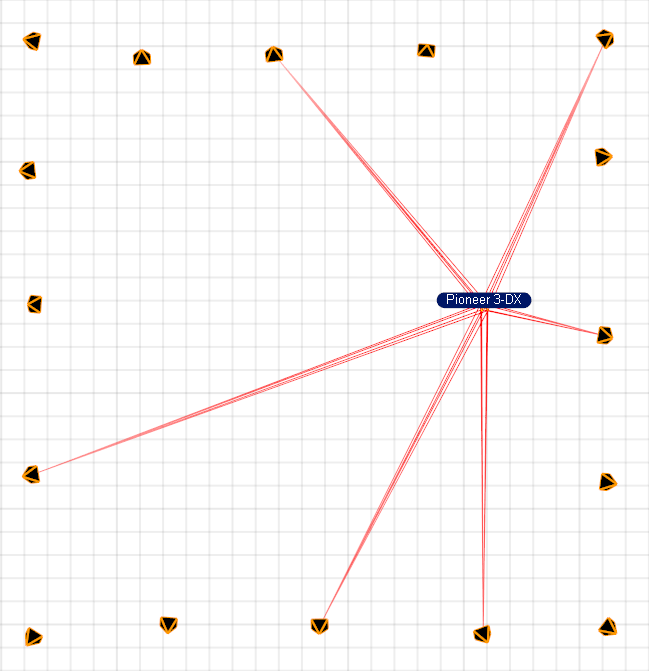
\includegraphics[width=0.75\textwidth]{gfx/mocap.png}
  \caption{Motion capture}
\end{figure}

For å posisjonere roboten i rommet ble det benyttet et motion capture system. Systemet var fast montert på rom
B333 og bestod av 16 infrarøde kamera av typen Flex 13 fra OptiTrack. Objekter som skulle spores ble utstyrt med markører som
reflekterte lys i det infrarøde området. Kameraene var utstyrt med infrarøde LED og hadde dermed mulighet til å posisjonere markørene i rommet. Ved å definere grupper av markører som stive
legemer kan systemet oppfatte både legemets posisjon og retning.

Et slikt system tilbød høy grad av presisjon, ned til få centimeter, men var også utsatt for støy i form av
lysforurensning. Området kameraene kunne spore et legeme var også
begrenset til noen få meter i hver retning fra midten av rommet.

Med kameraene fulgte det en programvarepakke som overførte posisjonen til de definerte legemene over nettverk
til datamaskinen som styrte roboten. Dataene ble importert i ROS og eksponert
som en topic. \graffito{Topics er ROS' implementasjon av meldingskanaler} Motion capture systemets
referanseramme samt posisjonen til roboten og posisjonen til brukeren ble overført på denne måten.

\section{Navigasjon}

\begin{figure}[!ht]
  \centering
  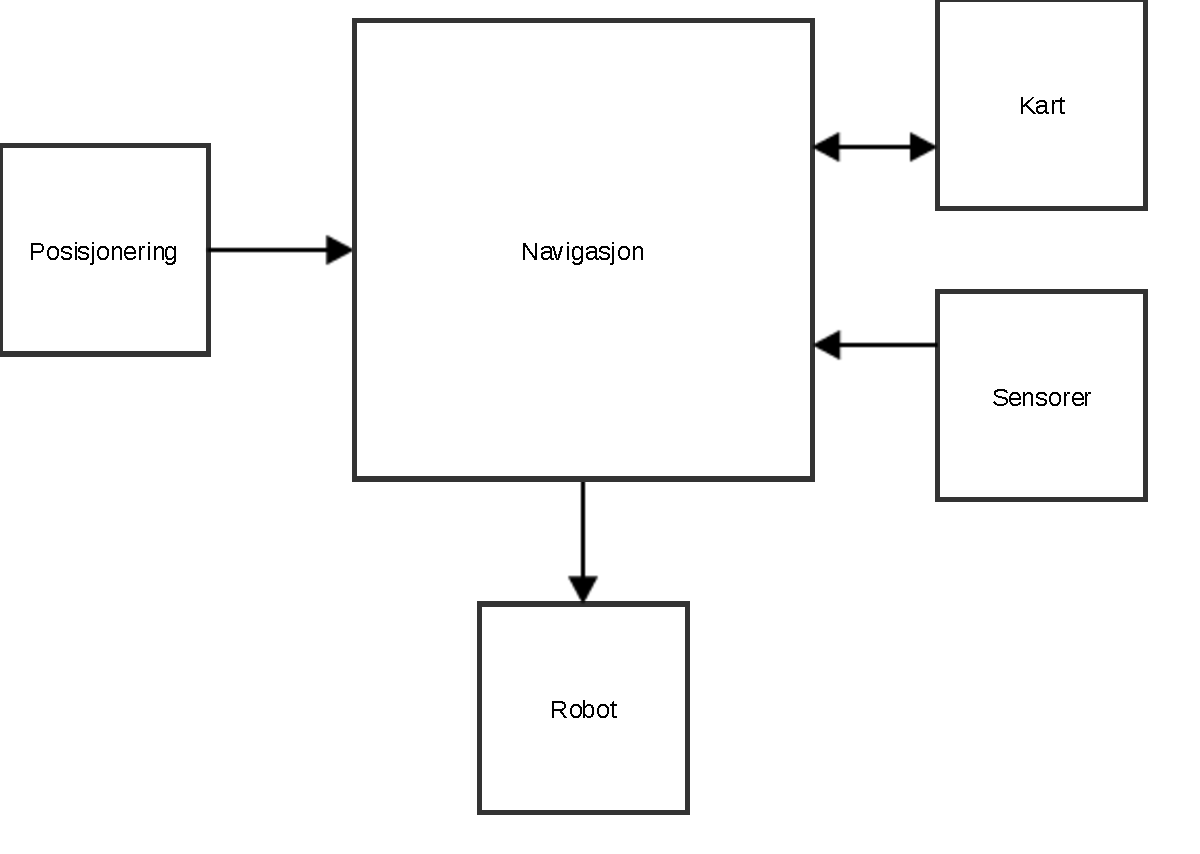
\includegraphics[width=\textwidth]{gfx/nav.pdf}
  \caption{Software stack}
  \label{fig:navstack}
\end{figure}

For å navigere roboten ble navigasjonspakken\footnote{\url{http://wiki.ros.org/navigation}} i ROS benyttet.
En oversikt over oppbygningen til denne pakken er vist i \autoref{fig:navstack}.
For å benytte dette systemet sammen med motion capture systemet ble systemets referanserammet overstyrt med den
fra motion capture anlegget, og inputkildene som kom inn fra venstre i \autoref{fig:navstack} var dermed ikke
relevante for den implementasjonen som ble benyttet.

Systemet mottok data fra lasermoduler og sonarmoduler for å orientere seg i forhold til hindringer i nærheten. 
Data fra sonar gav et lite detaljert bilde av omgivelsene, og var primært relevant for å detektere vegger
eller andre store hindringer. Laseren, vist i \autoref{fig:hokuyo}, hadde derimot oppløsning som gjorde at den kunne se også små hindringer. Knappene langs støtfangeren til roboten stanset bevegelse på et lavere nivå, slik at kjørekommandoer fra navigasjonssystemet ikke ble utført av roboten.

Ved bruk av sensordata fra laser og sonar bygde navigasjonssystemet et kostnadskart over omgivelsene, der hvert felt ble gitt
en verdi som indikerte kostnaden ved å forflytte seg gjennom feltet. Deretter benyttet systemet algoritmer for graftraversering
for å og benyttet dette da det planla en rute
frem til det gitte målet. Ruten ble planlagt i to stadier, globalt og lokalt. Den globale ruten ble generert
i det målet ble gitt til roboten, mens den lokale ruten ble oppdatert fortløpende etter som roboten tilegnet
seg ytterlige data om hindringer i omgivelsene. Om roboten møtte uforutsette hindringer forsøkte den å planlegge
en lokal rute rundt hindringen slik at den kom seg tilbake til den globale ruten. Om roboten etter en tid ikke
var i stand til å finne en slik rute vil den gi opp, og måtte gis et nytt mål før den kunne fortsette.

\begin{figure}[!ht]
  \centering
  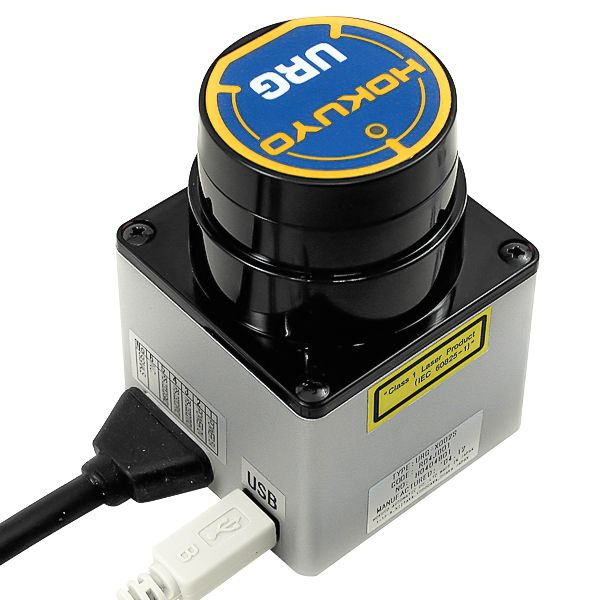
\includegraphics[width=0.5\textwidth]{gfx/hokuyo_urg_04lx.jpg}
  \caption[Hokuyo URG-04LX]{Hokuyo URG-04LX Scanning Laser Range Finder}
  \label{fig:hokuyo}
\end{figure}

For å gi roboten et mål å gå til ble to systemer utprøvd. Det første, for å teste funksjonalitet, bestod i å
gi roboten målpunkt ved å trykke på det ønskede målet i visualiseringsprogrammet RViz\footnote{\url{http://wiki.ros.org/rviz}}. Ved hjelp av dette var det på en enkel måte mulig å se hvordan
roboten tok seg frem til et mål, og hvordan den håndterte hindringer langs veien.
Et mer komplisert system som genererte målpunkter basert på bevegelsene til brukeren roboten skulle følge ble
også utprøvd, men aldri ferdigstilt i tilfredsstillende grad. Da
roboten bare kunne gis et mål av gangen bygde dette systemet en intern liste av målpunkter, og gav disse til
roboten ettersom roboten nådde det inneværende målpunktet. Dette ble implementert som en egen modul, knyttet sammen eksisterende moduler for å danne et komplett styringssystem til roboten. % Implementasjon
% Resultater

\chapter{Resultater} % Chapter title

\label{ch:resultater} % For referencing the chapter elsewhere, use \autoref{ch:mathtest}

% Formålet med dette kapittelet er å ta for oss målene og resultater som viser til at vi har oppnådd kravene til oppgaven.
%----------------------------------------------------------------------------------------
Kravene til systemet ble innført som moduler, og disse modulene ble implementert hver for seg. Disse omfatter styring og følging, kollisjonsdeteksjon og sikkerhet. Posisjonering av robot og menneske ble realisert ved bruk av infrarøde kamera og programvare fra OptiTrack. Stifinning, laser-mapping, sonar og generell motorkontroll av robot ble implementert ved bruk av programvare-rammeverket ROS. 
Vår prototype har liten form for sikkerhetstiltak utenom kollisjonsdetekesjon, hvor det var ønsket å kunne se på muligheter for å håndtere defekte sensorer og mulige situasjoner som ville ødelegge for handlevognen under kjøring.

De fleste modulene ble testet sammen, men det ble derimot ikke tid til å lage et fullstendig system som oppfylte spesifikasjonen vi hadde for konseptet autonom handlevogn.

En demonstrasjonsvideo\footnote{\url{https://www.youtube.com/watch?v=3kurIgqk0us}} ble laget for illustrere hvordan produktet skulle fungere i praksis. I videoen blir roboten styrt ved hjelp av en xbox-kontroller.  

\todo{Hva oppnådde vi med prosjektet?} % Resultater
% Chapter 7

\chapter{Diskusjon} % Chapter title

\label{ch:diskusjon} % For referencing the chapter elsewhere, use \autoref{ch:mathtest}

% Formålet med dette kapittelet er å diskutere resultatene, først og fremst mot teori og implementasjon.
%----------------------------------------------------------------------------------------

Som tidligere nevnt, så er resultatet av dette prosjektet i hovedsak et konsept, og ikke et ferdig produkt. Det har derimot blitt implementert en rekke programvaremoduler som ville ha vært nyttige for en eventuell realisering av et slikt konsept. Denne diskusjonsdelen vil derfor ta for seg funksjonaliteten til hver og en av disse modulene.

\section{Moduler}
\subsection{Posisjonering}

Posisjonering ble i dette prosjektet gjort ved hjelp av et Motion Capture system. Dette er en løsning som ville ha vært fullstendig urealistisk for en butikk å ta i bruk, da spesielt med tanke på pris. Ideelt sett så burde posisjonering av robot og menneske vært gjort ved å bruke en teknologitype som var mer tilgjengelig, slik som Bluetooth. Problemet med å bruke Bluetooth i dette prosjektet var i hovedsak knyttet opp i mot system som har tilgang på fasedata. 

\subsection{Stifinning}

I dette prosjektet ble stifinning implementert ved å bruke en ferdig modul fra programvare-rammeverket ROS. Den opprinnelige tanken var å implementere et liknende system selv, med oppbygning av et kostnadskart, og graf-traversering av dette ved hjelp av en algoritme som f.eks A*. Det viste seg å være vel så effektivt, og meget tidsbesparende, å benytte et ferdig softwareprodukt som gjorde akkurat dette.

\subsection{Kollisjonsdeteksjon}

Både laser-mapping og sonar ble tatt i bruk for å kunne kartlegge omgivelsene til roboten. Sonaren viste seg å være unøyaktig, og ble kun brukt til å vite om roboten var i nærheten av et hinder eller ikke. Laser-mappingen viste å være mye mer presis, og kunne brukes til å detektere langt mindre hindringer enn sonar kunne alene. Sammen utgjorde disse en effektiv løsning, slik at kollisjoner kunne unngås med tilfredsstillende grad av pålitelighet. De fysiske bryterene på robotens støtfanger fungerte som en siste utvei i tilfelle kollisjon, og hindret skade der navigasjonssystemet kom til kort.

\subsection{Sikkerhet}
Det ble liten tid til å begynne med sikkerhetstiltak. Dette er situasjoner utenom de øvrige kravene som gjør at roboten vil få problemer under kjøring. Vi ønsket å kunne oppdage om sensorer var defekte før eller under kjøring slik at den ville ha tiltak som gjorde den sikker i butikken. Muligheter ville vært å sende forespørsler ut til alle sensorer hvor de måtte gi gode verdier tilbake som tilsier noe om tilstanden. Hvis noe var feil ville roboten si ifra til kunde og komme seg tilbake til lagerområdet og sende beskjeder til ansatte over mobilapplikasjonen. Hvis kjøringsmotorikken var ødelagt ville den stoppet og sendt beskjeder til ansatte. % Diskusjon
% Konklusjon

\chapter{Konklusjon} % Chapter title

\label{ch:konklusjon} % For referencing the chapter elsewhere, use \autoref{ch:mathtest}

%  I dette kapittelet ønsker vi å uttrykke konklusjonene for vårt system.
% VIDERE ARBEID: Laserscanner informasjon er kun tilgjengelig via kablet ethernet. Dette burde bli gjort trådløst. 
% VIDERE ARBEID:
%----------------------------------------------------------------------------------------

Dette prosjektet har uten tvil bydd på sine utfordringer. Gruppen har hele tiden vært preget av en begrenset tidsramme, samt begrenset tilgang og kjennskap til nødvendige utviklingsverktøy. Dette tatt i betraktning til gruppens høye ambisjoner har gjort at selve produktet i sin fysiske form er ganske uferdig. På den andre siden så har det også gått med mye tid på planlegging, tilrettelegging og behovsanalyse av dette systemet. Det vi dermed står igjen med er derfor et svært spennende konsept som uten tvil har potensiale til kommersialisering. Dette resultatet stemmer også godt overens med vår resultatorienterte måloppnåelse, noe som synliggjøres av selve implementeringen. Gruppen velger derfor å betrakte prosjektet som vellykket, til tross for mangelen på en fullstendig implementasjon.  % Konklusjon
% Videre arbeid

\chapter{Videre arbeid} % Chapter title

\label{ch:viderearbeid} % For referencing the chapter elsewhere, use \autoref{ch:mathtest}

%  I dette kapittelet vil vi legge frem mulig videre arbeid og hva som eventuelt må gjøres før dette kan iverksettes. 
%----------------------------------------------------------------------------------------

Gjennom dette prosjektet har gruppen presentert et mulig konsept for en autonom handlevogn robot. Mye må likevel gjøres hvis produktet skal videreføres og eventuelt kommersialiseres. Dette kapittelet presenterer ulike forslag og synspunkter på en eventuell videreføring av konseptet.

Som tidligere nevnt i denne rapporten, så er pris en viktig suksessfaktor for et slikt produkt. Dagligvarebutikkene er på mange måter konservative, og lite villig til å investere dyrt i nye løsninger. Det er dessuten lite trolig at en utskiftning av ordinære handlevogner til fordel for autonome vil gi en stor økonomisk avkastning. Produktet bør først og fremst ansees som en mulighet for butikkene til å innføre et nytt sortiment av varer. En autonom handlevogn vil nemlig kunne åpne for å handle varer som tidligere ikke hadde vært mulig, på grunn av vekt eller størrelse. Dette er viktige betraktninger som bør tas hensyn til i en videre utvikling.

Posisjonering ble i dette prosjektet gjort ved hjelp av et motion capture system. Et slikt system er veldig presist, men er dyrt å anskaffe, spesielt for butikker som har et stort areal. En alternativ løsning til et slikt system anbefales derfor på sterkeste. Radiobasert posisjonering ved faseforskyvning kan f.eks. være et godt alternativ. Det ville også vært naturlig å forbedre posisjoneringen ved bruk av SLAM.

Et annet aspekt en må tenke på, er robotens intelligens. Bør den kunne følge dumt etter brukeren, eller bør den ha mulighet til å ta enkelte beslutninger på egen hånd. I et butikklokale kan det fort oppstå hindringer. Disse kan være lett for en person å unngå, men verre for en stor og tung robot. Roboten bør kanskje derfor ha en mulighet til å kunne foreta smarte valg, ved å finne alternative ruter og styre unna hindringer.

Det er for tiden et høyt fokus og satsning på selvkjørende biler. Mye av teknologien som utvikles på det området, vil kanskje være naturlig å ta i bruk i et slikt prosjekt. % Videre Arbeid


%----------------------------------------------------------------------------------------
%	THESIS CONTENT - APPENDICES
%----------------------------------------------------------------------------------------

%\appendix
%
%\part{Vedlegg} % New part of the thesis for the appendix
%
%\include{Chapters/appendix} % Appendix A

%----------------------------------------------------------------------------------------
%	POST-CONTENT THESIS PAGES
%----------------------------------------------------------------------------------------

\cleardoublepage% Bibliography

\label{app:bibliography} % Reference the bibliography elsewhere with \autoref{app:bibliography}

\manualmark
\markboth{\spacedlowsmallcaps{\bibname}}{\spacedlowsmallcaps{\bibname}} 
\refstepcounter{dummy}

\addtocontents{toc}{\protect\vspace{\beforebibskip}} % Place the bibliography slightly below the rest of the document content in the table of contents
\addcontentsline{toc}{chapter}{\tocEntry{\bibname}}

\bibliographystyle{plainnat}

\bibliography{Bibliography} % Bibliography

\cleardoublepage\include{FrontBackMatter/Colophon} % Colophon

\cleardoublepage\include{FrontBackMatter/Declaration} % Declaration

%----------------------------------------------------------------------------------------

\end{document}
